\section{DIS projections for LHC far-forward experiments}
\label{sec:dis_pseudodata}

Here we describe the procedure adopted in order 
to generate projections for the kinematic coverage
and experimental uncertainties associated to  measurements
of neutrino-nucleus scattering at the LHC far-forward experiments.
%
First, we summarise the theoretical description of differential
neutrino scattering in terms of DIS structure functions and highlight
their PDF sensitivity.
%
Second, we present an  overview of the operative and proposed
LHC far-forward neutrino detectors that
will be considered in the present study and indicate their
main acceptance and performance parameters.
%
By convoluting the expected muon neutrino fluxes
with the acceptance and scattering rates of each
of these detectors,
we evaluate the foreseen event yields in bins of $x$, $Q^2$,
and $E_\nu$ and therefore the associated statistical uncertainties.
%
We also estimate how the systematic uncertainties in the measurement
of final-state variables affects the experimental covariance matrix. 

\subsection{Neutrino DIS revisited}

The double-differential cross-section for neutrino-nucleus charged-current scattering,
see~\cite{Candido:2023utz} and references therein,
is expressed in terms of 
independent structure functions $F_2^{\nu A}$, $xF_3^{\nu A}$
and $F_L^{\nu A}$:
\be
\label{eq:neutrino_DIS_xsec_FL}
\frac{d^2\sigma^{\nu A}(x,Q^2,y)}{dxdy} =  \frac{G_F^2s/4\pi}{\lp 1+Q^2/m_W^2\rp^2}\lc Y_+F^{\nu A}_2(x,Q^2) - y^2F^{\nu A}_L(x,Q^2) +Y_- xF^{\nu A}_3(x,Q^2)\rc  \, ,
\ee
where $Y_\pm = 1 \pm (1-y)^2$ and with a counterpart expression for anti-neutrino scattering,
\be
\label{eq:antineutrino_DIS_xsec_FL}
\frac{d^2\sigma^{\bar{\nu} A}(x,Q^2,y)}{dxdy} =  \frac{G_F^2s/4\pi}{\lp 1+Q^2/m_W^2\rp^2}\lc Y_+F^{\bar{\nu} A}_2(x,Q^2) - y^2F^{\bar{\nu} A}_L(x,Q^2) -Y_- xF^{\bar{\nu} A}_3(x,Q^2)\rc  \, ,
\ee
where $s=2m_N E_\nu$ being the neutrino-nucleon center of mass energy squared, $m_N$ is the nucleon mass,
$E_\nu$ is the incoming neutrino energy,
and the inelasticity is $y=Q^2/(2x m_n E_{\nu})$.
%
Structure functions depend only on $x$ and $Q^2$ while the differential
cross-section depends also on the neutrino energy $E_\nu$, or alternatively
on the inelasticity $y$.
%
Further, structure functions $F^{\nu A}_i(x,Q^2)$ and $F^{\bar{\nu} A}_i(x,Q^2)$ depend on the nuclear target $A$ entering
for the neutrino scattering through the nuclear modifications of the proton PDFs.

Eqns.~(\ref{eq:neutrino_DIS_xsec_FL}) and~(\ref{eq:antineutrino_DIS_xsec_FL}) are valid provided
the hadronic 
invariant mass $W$  is above the resonance threshold,
\be
W^2 = \lp m_N^2 + Q^2 \frac{(1-x)}{x} \rp \gsim \lp 2\,{\rm GeV} \rp^2\, ,
\ee
and in addition here we  restrict ourselves to the DIS region with perturbative momentum
transfers $Q^2$, such that
 structure functions are decomposed as
\be
\label{eq:sfs_pqcd}
 F^{\nu A}_i(x,Q^2) = \sum_{j=q,\bar{q},g}\int_x^1 \frac{dz}{z}\, C_{i,j}^{\nu N}(z,\alpha_s(Q^2))f^{(A)}_j\lp \frac{x}{z},Q^2\rp \, , \quad i = 2,3,L \, .
 \ee
%
in terms of a convolution of partonic scattering cross-sections  $C_{i,j}^{\nu N}(x,\alpha_s)$ and
of process-independent PDFs $f^{(A)}_j\lp x,Q^2\rp$.
%
Specifically, in this work we impose that $Q^2\ge 2$ GeV$^2$.
%
A similar expression holds for charm production~\cite{Faura:2020oom}, which requires
accounting also for charm mass effects~\cite{Gao:2017kkx}.
 %
We discuss in Sect.~\ref{sec:settings} the theoretical
settings adopted~\cite{Candido:2022tld,yadism,Candido:2023utz,Carrazza:2020gss} to
evaluate predictions for
neutrino DIS structure functions
and differential cross-sections,
Eqns.~(\ref{eq:neutrino_DIS_xsec_FL}),~(\ref{eq:antineutrino_DIS_xsec_FL}), and~(\ref{eq:sfs_pqcd}),
in the kinematics covered by LHC neutrinos.

Different neutrino structure functions provide complementary sensitivity
 to the partonic flavour decompositions of nucleons.
 %
 To illustrate this sensitivity, consider a leading order  calculation
 for a proton target with $n_f=4$ active quark flavours,
a diagonal CKM matrix and no heavy quark mass effects.
 %
 The resulting $F_2^{\nu p}$ and $xF_3^{\nu p}$ structure functions read
 \bea
 F_2^{\nu p}(x,Q^2) &=& 2x\lp f_{\bar{u}} + f_{d} + f_{s} + f_{\bar{c}} \rp(x,Q^2) \, , \nonumber  \\
 F_2^{\bar{\nu} p}(x,Q^2) &=& 2x\lp f_u + f_{\bar{d}} + f_{\bar{s}} + f_c \rp(x,Q^2) \, , \label{eq:neutrinoSFs_proton} \\
 xF_3^{\nu p}(x,Q^2) &=& 2x\lp -f_{\bar{u}} + f_d +f_s - f_{\bar{c}}\rp(x,Q^2)  \, , \nonumber\\
 xF_3^{\bar{\nu} p}(x,Q^2) &=& 2x\lp f_u - f_{\bar{d}} -f_{\bar{s}} + f_{c}\rp(x,Q^2) \, . \nonumber
 \eea
 The corresponding expressions for a neutron target are obtained from isospin symmetry
 \bea
 F_2^{\nu n}(x,Q^2) &=& 2x\lp f_{\bar{d}} + f_{u} + f_{s} + f_{\bar{c}} \rp(x,Q^2) \, , \nonumber  \\
 F_2^{\bar{\nu} n}(x,Q^2) &=& 2x\lp f_d + f_{\bar{u}} + f_{\bar{s}} + f_c \rp(x,Q^2) \, , \label{eq:antineutrinoSFs_neutron} \\
 xF_3^{\nu n}(x,Q^2) &=& 2x\lp -f_{\bar{d}} + f_u +f_s - f_{\bar{c}}\rp(x,Q^2)  \, , \nonumber\\
 xF_3^{\bar{\nu} n}(x,Q^2) &=& 2x\lp f_d - f_{\bar{u}} -f_{\bar{s}} + f_{c}\rp(x,Q^2) \, , \nonumber
 \eea
 while for an isoscalar, free-nucleon target denoted by $N$ one has
 \bea
 F_2^{\nu N}(x,Q^2) &=& 2x\lp f_{u^+} + f_{d^+} + 2f_s + 2f_{\bar{c}} \rp(x,Q^2) \, , \nonumber  \\
 F_2^{\bar{\nu} N}(x,Q^2) &=& 2x\lp f_{u^+} + f_{d^+} + 2f_{\bar{s}} + 2f_c \rp(x,Q^2) \, , \label{eq:neutrinoSFs_isoscalar} \\
 xF_3^{\nu N}(x,Q^2) &=& 2x\lp f_{u^-} + f_{d^-} +2f_s - 2f_{\bar{c}}\rp(x,Q^2)  \, , \nonumber\\
 xF_3^{\bar{\nu} N}(x,Q^2) &=& 2x\lp   f_{u^-} + f_{d^-}-2f_{\bar{s}} +2 f_{c}\rp(x,Q^2) \, , \nonumber
 \eea
 in terms of the valence and sea PDF combinations defined by
 \be
 f_{q^+} (x,Q^2)\equiv \lp f_{q}+f_{\bar{q}}\rp(x,Q^2) \, , \qquad
 f_{q^-} (x,Q^2)\equiv \lp f_{q}- f_{\bar{q}}\rp(x,Q^2) \, .
 \ee
 We note that, even for isoscalar targets, separate measurements
 for neutrinos and antineutrinos will not be equivalent, since in general
 the strange and charm sea asymmetries $f_{s^-}$ and
 $f_{c^-}$ are not expected to vanish.

 In the projections presented in this work, when interpreting the LHC neutrino structure
 functions in terms of proton PDFs, we will assume a isoscalar free-nucleon target and neglect
 nuclear PDF modifications, along the lines of Eq.~(\ref{eq:neutrinoSFs_isoscalar}).
 %
 On the other hand, when evaluating structure functions
 for a tungsten (W) target, we keep into account both
 nuclear corrections and that
 the target is not isoscalar when evaluating the physical observables.
 %
 We point out that accounting for nuclear modifications in a global proton
 PDF fit is possible by means of the procedure developed
 in~\cite{Ball:2020xqw,Ball:2018twp}.

 It is illustrative to compare the PDF dependence of neutrino structure functions
 at LO with that of their counterparts for neutral-current
 scattering with a charged lepton projectile.
 %
 Within the same assumptions, for energies below
 the $Z$-boson mass, $Q^2 \ll m_Z^2$, the corresponding
 partonic decomposition is
 the 
 \bea
 F_2^{\ell p}(x,Q^2) &=& x\lp \frac{4}{9}\lc f_{u^+} + f_{c^+}\rc
 + \frac{1}{9}\lc f_{d^+} + f_{s^+}\rc\rp(x,Q^2) \, , \nonumber  \\
 F_2^{\ell n}(x,Q^2) &=& x\lp \frac{4}{9}\lc f_{d^+} + f_{c^+}\rc
 + \frac{1}{9}\lc f_{u^+} + f_{s^+}\rc\rp(x,Q^2) \, ,\label{eq:NC_chargedlepton}   \\
 F_2^{\ell N}(x,Q^2) &=& x\lp \frac{5}{18}\lc f_{u^+} + f_{d^+}\rc
 + \frac{1}{9} f_{s^+} + \frac{4}{9} f_{c^+} \rp(x,Q^2) \, , \nonumber  
 \eea
 with $xF_3$ being negligible in this region below the $Z$-pole.
 %
 Eq.~(\ref{eq:NC_chargedlepton}) showcases the complementarity between
 neutrino and charged-lepton DIS in terms of sensitivity
 to the different flavour PDF decomposition.

 \subsection{Far-forward neutrino detectors at the LHC}
 \label{sec:neutrinoDetectors}

 The calculation of differential neutrino scattering event rates
 at the LHC far-forward detectors involves two main ingredients: the energy
 and flavour dependence of the incoming neutrino flux crossing
 the detector fiducial volume, on the one hand,
 and the scattering rates within the same fiducial volume, on the other hand.
 %
 In this section, we summarise the main features of each of the existing and future
 far-forward detectors considered in this study, in particular concerning
 their acceptance, performance, and detection method.
 %
 We focus on  muon
 neutrino scattering, which benefits from the highest rates and is less
 affected by uncertainties affecting $D$-meson production.
 
 The kinematics of a charged-current neutrino DIS event $(x,Q^2, E_\nu)$,
 or alternatively $(x,Q^2, y)$, are uniquely specified by the measurement of three independent
 final-state variables,
 such as $\lp E_\ell,\theta_\ell, W^2\rp$ or $\lp E_\ell,\theta_\ell, E_h \rp$,
 with $E_\ell$ and $\theta_\ell$ being the energy and polar angle of the outgoing
 charged lepton and $E_h$ the total energy of the hadronic final state.
 %
 Most neutrino detectors can only access $E_h$, given that $W^2$ requires
 fully reconstructing this final state.
 %
 A measurement of  $\lp E_\ell,\theta_\ell, E_h \rp$ then fixed the DIS kinematics as:
 \bea
 E_\nu &=& E_h + E_\ell \, , \nonumber \\
 Q^2 &=& 4 ( E_h + E_\ell) E_\ell \sin^2 \lp \theta_\ell/2\rp \, ,  \label{eq:dis_kinematic_mapping}\\
 x&=& \frac{4 ( E_h + E_\ell) E_\ell \sin^2 \lp \theta_\ell/2\rp}{2m_N E_h} \, .\nonumber
 \eea
 These relations also indicate how systematic uncertainties affecting the measurement
 of $\lp E_\ell,\theta_\ell, E_h \rp$ translate into uncertainties in the
 reconstructed values of  $(x,Q^2, E_\nu)$, which in turn modify the expected
 event rates in a given bin.

 Table~\ref{tab:FPF_experiments} indicates,
for each of the far-forward LHC neutrino experiments considered
  in this work,  their neutrino pseudo-rapidity coverage, target material, whether
  they can identify the sign of the outgoing charged lepton,
  the acceptance for the charged lepton and hadronic final state,
  and the expected reconstruction performance.
  %
  We consider separately acceptance and performance for electron and muon
  neutrinos, while tau neutrinos have lower production rates and are neglected in this study.
  %
  For these projections we assume that FASER$\nu$ and SND@LHC acquire data
  for the full Run III period, while FASER$\nu$2, AdvSND, and FLArE take data
  for the complete HL-LHC period.
  %
  An estimate of the expected 
  systematic uncertainties is not available for FASER$\nu$ and SND@LHC, experiments
  which are nevertheless limited by statistics.
  %
  In the following we provide more details about the information collected in
  Table~\ref{tab:FPF_experiments}.

%---------------------------------------------------
    %-----------------------------------------------------------------
\begin{table}[t]
  \centering
  \small
  \renewcommand{\arraystretch}{1.50}
\begin{tabularx}{\textwidth}{Xccccc}
\toprule
Detector &  Rapidity &  Target & Charged Lepton ID & Acceptance  & Performance \\
\midrule
\midrule
\multirow{3}{*}{FASER$\nu$}  &  \multirow{3}{*}{ $\eta_\nu \ge 8.5$}  &   \multirow{2}{*}{Tungsten}  & \multirow{3}{*}{muons}      &   $E_\ell \gsim 100$ GeV   &      $\delta E_\ell \sim 30\% $    \\
&   &   \multirow{2}{*}{(1.1 ton)}  &       &  $\tan \theta_\ell \lsim 0.025$   &
$\delta \theta_\ell \sim 0.06$ mrad        \\
&   &     &       &  reconstructed $E_h$ \& charm ID   &      $\delta E_h \sim 30\%$     \\
\midrule
\multirow{2}{*}{SND@LHC}  & \multirow{2}{*}{ $7.2 \le \eta_\nu \le 8.4$}   &  Tungsten   &   \multirow{2}{*}{n/a}    &  $E_\mu \gsim 20 $ GeV     &    \multirow{2}{*}{n/a}    \\
  &    &  (0.83 ton)   &  &  $\theta_\mu \lsim 0.15, \theta_e \lsim 0.5$         &       \\
\midrule
\midrule
\multirow{3}{*}{FASER$\nu$2}  & \multirow{3}{*}{ $\eta_\nu \ge 8.5$}  & \multirow{2}{*}{Tungsten}    &   \multirow{3}{*}{muons}     &   $E_\ell \gsim 100$ GeV  &    $\delta E_\ell \sim 30\% $     \\
  &   &  \multirow{2}{*}{(20 ton)}   &       &  $\tan \theta_\ell \lsim 0.05$   &   $\delta \theta_\ell \sim 0.06$ mrad      \\
  &   &     &       &  reconstructed $E_h$ \& charm ID   &  $\delta E_h \sim 30\%$        \\
\midrule
\multirow{3}{*}{AdvSND-far}  &   \multirow{3}{*}{ $7.2 \le \eta_\nu \le 8.4$}  &
\multirow{2}{*}{Tungsten}   &   \multirow{3}{*}{muons}    &  $E_\mu \gsim 20 $ GeV  & \multirow{3}{*}{n/a}          \\
  &   &   \multirow{2}{*}{(5 ton)}  &        & $\theta_\mu \lsim 0.15, \theta_e \lsim 0.5$     &           \\
  &   &     &       &  reconstructed $E_h$   &           \\
\midrule
\multirow{3}{*}{FLArE ({\bf *})}  & \multirow{3}{*}{$\eta_\nu \ge 7.5$} & \multirow{2}{*}{LAr}  & \multirow{3}{*}{muons}  &  $E_\mu \gsim 2$ GeV, $E_e \lsim 2$ TeV    &    $\delta E_e \sim 5\% $ \\
&   &  \multirow{2}{*}{(10 ton)}   &   & $\theta_\mu \lsim 0.025$, $\theta_e \lsim 0.5$ &    $\delta \theta_e \sim 15 $ mrad   \\
 &   &     &  & reconstructed $E_h$  &    $\delta E_h \sim 30\% $   \\
  \bottomrule
\end{tabularx}
\vspace{0.2cm}
\caption{\small For each of the far-forward LHC neutrino experiments considered
   we indicate their neutrino pseudo-rapidity coverage, target material, whether
  they can identify the sign of the outgoing charged lepton,
  the acceptance for the charged lepton and hadronic final state,
  and the expected reconstruction performance.
  %
  We consider separately acceptance and performance for electron and muon
  neutrinos.
  %
  For FLArE, we assume that muons would be measured in the FASER2 spectrometer
  situated downstream in the FPF cavern.
  %
  See the description of each experiment in the text for more details.
  %
  For our projections we assume that FASER$\nu$ and SND@LHC acquire data
  for the Run III period ($\mathcal{L}=150$ fb$^{-1}$), while FASER$\nu$2, AdvSND, and FLArE take data
  for the complete HL-LHC period ($\mathcal{L}=3$ ab$^{-1}$).
  %
  In the case of FLArE, we consider results both
  for 10 ton and 100 fiducial volume detectors.
  \label{tab:FPF_experiments}
}
\end{table}
%-----------------------------------------------------------------

%---------------------------------------------------

\paragraph{FASER$\nu$.}
%
The ForwArd Search ExpeRiment (FASER) detector and its companion FASER$\nu$~\cite{FASER:2019aik,FASER:2019dxq}
are located at the TI12 tunnel of the CERN accelerator complex.
%
Both detectors are aligned
with the collision axis line-of-sight (LOS)
and have been acquiring data since the begin of Run III.
%
Neutrino scattering takes place in the FASER$\nu$
detector, composed by interleaved emulsion and tungsten plates and
adding up to a mass of 1.1 tons with a fiducial volume of $20~\rm{cm} \times 25~\rm{cm} \times 30~{\rm cm}$.
%
The FASER apparatus is immersed in a magnetic field  providing charged lepton
identification thanks to two 1 m-long dipole magnets with $B=0.57$ T
and another 1.5 m-long magnet in front of the spectrometer. 
%
Neutrino detection and identification can be carried out either using the emulsion
films of FASER$\nu$2, which have the key benefit of excellent position and angular resolution,
or instead using the electronic detector components of FASER, which enable the tagging
of the outgoing downstream energetic muons.

\paragraph{SND@LHC.}
%
In the same manner as FASER, the SND@LHC experiment is located in a service tunnel (TI18)
around 500 meters from the ATLAS interaction point and has been taking data
since the  beginning of Run 3.
%
SND@LHC is installed off the LOS axis in order to cover the neutrino
pseudo-rapidity range of $7.2 \le \eta_\nu \le 8.4$.
%
With a total fiducial volume of 830 kg, it is composed by tungsten plates,
where neutrino scattering takes place, interleaved with nuclear emulsions and electronic tracker
components.
%
Downstream, the scattering volume is followed by a hadronic calorimeter and a muon tracking system.
%
The electromagnetic
 and hadronic energy deposits can be measured at the electronic detectors, with the emulsion
 components providing vertex reconstruction.
 %
 The lack of magnetic field prevents the charge-sign identification of the outgoing charged leptons.

\paragraph{FASER$\nu$2.}
%
A proposed 20-ton neutrino experiment located on the LOS
of the LHC neutrino beam to be installed in the FPF cavern.
%
It is based on an emulsion-based detector optimised to identify heavy flavor particles, including
tau leptons and charm and beauty particles, arising from neutrino interactions.
%
The FASER$\nu$2 detector is composed of 3300 emulsion layers interleaved with 2-mm-thick tungsten plates,
for a total volume of  tungsten of $40~\rm{cm} \times 40~\rm{cm} \times 6.6~{\rm m}$.
%
The combination of FASER$\nu$2  with the nearby FASER2 detector, equipped with a spectrometer, makes measurements of the outgoing muon charge possible.

 \paragraph{AdvSND.}
 %
 This experiment consists on  two detectors, a far-detector to be installed
 at the FPF with a coverage in neutrino pseudorapidity $\eta_\nu$ of $7.2 \le \eta_\nu \le 8.4$
 (hence off-LOS) and a near detector installed somewhere else in LHC
 complex and covering the range $4 \le \eta_\nu \le 5$.
 %
 In the following we focus on the AdvSND far-detector.
 %
 It would be
 composed (from upstream to downstream) by a target region
 for  vertex reconstruction and electromagnetic energy measurement, followed  by a hadronic calorimeter, a  muon identification system, and finally  a magnet enabling muon charge and momentum measurements.
 %
 The target region of the detector, where the neutrino interactions take place, is made of thin sensitive layers interleaved with tungsten plates, for a total mass of 5 tons.
 %
 This detector configuration will be able to track muons with energy $E_\nu \gsim 20$ GeV
 within an acceptance of 100 mrad and provide information on the charge
 of the  outgoing muon thanks to its magnet.
 %
 The total energy of the hadronic final state will be measured
 in the hadronic calorimeter.

 \paragraph{FLArE.}
 %
 Building upon recent progress in liquid noble gas neutrino detectors over the last decade (ICARUS, MicroBooNE, SBND, ProtoDUNE, DUNE), this experiment relies on a modularized liquid argon (LAr) time projection detector.
 %
 The use of LAr as target is beneficial for final-state particle identification, track angle, and kinetic energy measurements with sub-millimeter spatial resolution in all three dimensions.
 %
 FLArE is suitable to identify high-energy neutrinos ($E_\nu \gsim 100$ GeV)  from all three generations
 while  fully containing the events as required for kinematic reconstruction.
 %
 The detector will be equipped with a magnetized hadron/muon calorimeter downstream of the liquid argon volume
 for muon charge and momentum measurements.
 %
 With an expected fiducial (active) mass of 10 tons (30 tons), FLArE will
 detect final-state electrons with energies $E_{e}\lsim 1~\rm{TeV}$ and
 scattering angles up to 0.5 mrad, while detecting final-state muons
 is restricted to $E_{e}\lsim 2~\rm{GeV}$  and $\theta_\mu \lsim 0.4$.
 %
 Reconstruction of the total energy of the hadronic final state will also
 possible. 
 %
 In terms of performance, the targets
 are $\delta E_\mu \sim$5\% of electron energy resolution,
 $\delta \theta_e \sim 15$ mrad of electron angular  resolution,
 and $\delta E_h \sim 30$\% for the hadronic energy.

\subsection{Differential event rate calculation}
\label{sec:pseudo-data_generation}

For each of the LHC far-forward neutrino detectors
described in Table~\ref{tab:FPF_experiments}, we generate
projections for the expected precision of DIS structure function
measurements as follows.
%
The goal is to evaluate the number of reconstructed charged-current neutrino interaction
events taking place in the fiducial volume of the detector in bins of Bjorken-$x$,
momentum transfer $Q^2$, and neutrino energy $E_\nu$, that is,
\be
\label{eq:event_yields}
N_{\rm ev}^{(i)}\lp \nu_e ; E_{{\rm min}}^{(i)} \le E_\nu \le E_{{\rm max}}^{(i)} ,\,
x_{{\rm min}}^{(i)} \le x \le x_{{\rm max}}^{(i)} ;\, Q_{{\rm min}}^{2(i)} \le Q^2 \le Q_{{\rm max}}^{2(i)}\rp
\, ,\quad i=1,\ldots, N_{\rm bins} \, ,
\ee
for electron neutrinos and for each of the bins composing the measurement, and with similar
expressions applying for muon and tau neutrinos and antineutrinos.
%
These event yields determine the statistical
precision associated to a measurement of the double-differential cross-sections
Eqns.~(\ref{eq:neutrino_DIS_xsec_FL}) and~(\ref{eq:antineutrino_DIS_xsec_FL}).
%
Subsequently, we account for the expected reconstruction performance of the detector
in order to estimate the systematic uncertainties associated to these event yields.
%
The choice of the binning is in principle arbitrary, and here we define them
to ensure that Gaussian statistics hold for all the bins of the measurement.

In this calculation, we assume the central values of the neutrino fluxes provided by the calculation
of~\cite{Kling:2021gos}.
%
The bin-by-bin integrated event yields in Eq.~(\ref{eq:event_yields}) are
obtained by convoluting the incoming neutrino fluxes, for a given geometric acceptance
of the target detector, with the corresponding neutrino differential cross-sections
Eqns.~(\ref{eq:neutrino_DIS_xsec_FL}) and~(\ref{eq:antineutrino_DIS_xsec_FL}).
%
As we further discuss in Sect.~\ref{sec:settings}, theoretical predictions
for the latter are computed with {\sc\small YADISM} interfaced to {\sc\small PineAPPL}
to produce fast precomputed interpolation grids.
%
Differential event yields are therefore evaluated using
\begin{equation}
  \label{eq:event_yields}
   N_{\rm ev}^{(i)} = n_T L_T\int_{Q^{2(i)}_{\rm min}}^{Q^{2(i)}_{\rm max}}\int_{x^{(i)}_{\rm min}}^{x^{(i)}_{\rm max}}\int_{E_{\rm min}^{(i)}}^{E_{\rm max}^{(i)}} \frac{dN_{\nu}(E_\nu)}{dE_{\nu}}\left(\frac{d^2\sigma(x,Q^2,E_{\nu})}{dxdQ^2}\right) {\cal A}(x,Q^2,E_{\nu}) dQ^2 dx dE_{\nu} \, ,\quad i=1,\ldots, N_{\rm bins} \, ,
\end{equation}
with $n_T$ is the nuclear density of the target detector material, $L_T$ its length and ${\cal A}(x,Q^2,E_{\nu})$ is an acceptance factor which takes the form of a step function and accounts for the experimental thresholds from Table\ref{tab:FPF_experiments}.
%
The incoming neutrino fluxes, which include the geometric acceptance of the considered detector,
are encoded in $dN_{\nu}(E_\nu)/dE_{\nu}$.
%
We consider only the scattering of muon neutrinos, characterised by the highest rates.
%
We verify that the differential event yield calculation
implemented in Eq.~(\ref{eq:event_yields}), when extrapolated to a single bin
covering the full detector acceptance,
is consistent with the fiducial interaction rates presented in~\cite{Feng:2022inv}.

The triple integral in  Eq.~(\ref{eq:event_yields}) is evaluated numerically by means
of Monte Carlo sampling, by generating sampling $N_{\rm mc}$ points in the $\lp x,Q^2,E_{\nu}\rp$ space
with the constraint that $0 < y = Q^2/2m_N E_{\nu }x <1 $
and then  integrating over the bin range:
\begin{equation}
    N_{\rm ev}^{(i)} \approx n_T L_T \frac{(Q^{2(i)}_{\rm max}-Q^{2(i)}_{\rm min})(x^{(i)}_{\rm max}-x^{(i)}_{\rm min})(E_{\rm max}^{(i)}-E_{\rm min}^{(i)})}{N_{\rm mc}}\times \sum_{j=1}^{N_{\rm mc}} \frac{dN_{\nu}(E^{(j)}_\nu)}{dE_{\nu}}\left(\frac{d^2\sigma(x^{(j)},Q^{2(j)},E^{(j)}_{\nu})}{dxdQ^2}\right) {\cal A}(x^{(j)},Q^2^{(j)},E_{\nu}^{(j)}) \, ,
    \label{MCintegration}
\end{equation}
and where $N_{\rm mc}$ is chosen to be large enough such that residual Monte Carlo integration
uncertainties are negligible for all the bins considered.

Table~\ref{tab:integrated_rates} summarises the predicted integrated event yields for the five detectors
considered, separated into electron neutrinos and antineutrinos
  and muon neutrinos and antineutrinos.
  %
  These event yields are computed from Eq.~(\ref{eq:event_yields}) with the only
  requirement that the momentum transfer and the final-state invariant mass are restricted
  to the DIS region,
  \be
  \label{eq:DISconditions}
Q^2 \ge 2~{\rm GeV}^2\quad{\rm and}\quad  W^2 \ge 4~{\rm GeV}^2 \, .
\ee
  %
   The numbers in parenthesis indicate the event rates corresponding to charm
  production, for those experiments with heavy flavour tagging capabilities.

%----------------------------------------------------
%%%%%%%%%%%%%%%%%%%%%%%%%%%%%%%%%%%%%%%%%%%
%-----------------------------------------------------------------
\begin{table}[t]
  \centering
  \small
  \renewcommand{\arraystretch}{1.70}
\begin{tabularx}{\textwidth}{X|c|c|c|c|c|c}
\toprule
Detector & $\quad$ $N_{\nu_e}$ $\quad$ &$\quad$ $N_{\bar{\nu}_e}$$\quad$   &   $N_{\nu_e} + N_{\bar{\nu}_e}$ &
$\quad$$N_{\nu_\mu}$ $\quad$ & $\quad$ $N_{\bar{\nu}_\mu}$ $\quad$  &   $N_{\nu_\mu} + N_{\bar{\nu}_\mu}$ \\
\midrule
\midrule
FASER$\nu$  & 620 (89)    & 220 (41)  & 850 (130)  &  1700 (230)  &  480 (84)  &  2200 (320) \\
SND@LHC  &  120 (15)  & 60 (9)    &180 (24)   &  450 (54) & 160 (22)   &  610  (76)\\
\midrule
\midrule
FASER$\nu$2  &    &    &   & 115000 (15700)  & 27000 (4700)    & 142000 (19700)   \\
AdvSND-far  &    &    &   &   &    &    \\
FLArE & 15100 (1800) & 7900 (1200)   &  22400 (1900) &  101000 (12200)&   30400 (4100) &   131000 (16300) \\
  \bottomrule
\end{tabularx}
\vspace{0.2cm}
\caption{\small Integrated event yields for the five detectors considered,
  separated into electron neutrinos and antineutrinos,
  muon neutrinos and antineutrinos, and their sum.
  %
  These event yields are computed from Eq.~(\ref{eq:event_yields_calculation})
  imposing DIS kinematics, $Q^2 \ge 2$ GeV$^2$ and $W^2 \ge 4$ GeV$^2$.
  %
  Whenever available, the
  numbers in parenthesis indicate the event rates corresponding to charm
  production.
  \label{tab:integrated_rates}
}
\end{table}
%-----------------------------------------------------------------
%%%%%%%%%%%%%%%%%%%%%%%%%%%%%%%%%%%%%%%%%%%%

%----------------------------------------------------

Eq.~(\ref{eq:event_yields}) can be generalised to charm-production events, with
the only difference being that now the neutrino scattering cross-section is restricted
to those processes leading to final-state charm quarks.
%
Assuming that charm quarks can be directly tagged by the detector one has
\be
\label{eq:event_yields_charm}
  N_{\rm ev,c}^{(i)} = n_T L_T\int_{Q^{2(i)}_{\rm min}}^{Q^{2(i)}_{\rm max}}\int_{x^{(i)}_{\rm min}}^{x^{(i)}_{\rm max}}\int_{E_{\rm min}^{(i)}}^{E_{\rm max}^{(i)}} \frac{dN_{\nu}(E_\nu)}{dE_{\nu}}\left(\frac{d^2\sigma^{\nu N \to \ell + c+X}(x,Q^2,E_{\nu})}{dxdQ^2}\right) dQ^2 dx dE_{\nu} \, 
  \ee
  with the charm production cross-sections discussed in~\cite{Faura:2020oom}
  and references therein.
  %
  Detectors without charm-tagging capabilities can still be sensitive to charm production via
  the semileptonic decays of the $D$-mesons, resulting in the characteristic
  dimuon topology, where
  \be
 N_{\rm ev,2\mu}^{(i)} \approx N_{\rm ev,c}^{(i)} \times \mathcal{B}\lp c \to D \to \mu + X\rp \, ,
 \ee
 with $\mathcal{B}$ a numerical factor that accounts for charm hadronisation and the
 resulting semileptonic decay to a muon.
 %
 Given that $\mathcal{B}\sim 0.1$, being able to tag directly charm quarks increases the event yields
 of charm production events by a factor of 10 as compared to reconstructing the dimuon final state.
 %
 Here we neglect finite acceptance effects, which can only be properly estimated by means
 of a full detector simulation.

 Fig.~\ref{fig:fasernu2_muon} displays the
 event yields per bin,  Eq.~(\ref{eq:event_yields}),
  for muon neutrinos detected at FASER$\nu$2 restricted
  to the DIS region defined by Eq.~(\ref{eq:DISconditions}).
  %
  We present results binned in $x$ and $Q^2$ and integrated over all available neutrino energies.
  %
  The red dot indicates the weighted center of each bin.
  %
  Adding up all bin entries results into the $N_{\nu_\mu}$ value
  for reconstructed muon
  neutrinos listed in
  Table~\ref{tab:integrated_rates}.
  %
  Only bins with at least 30 events are retained, to ensure the validity of Gaussian
  statistics.
  %
  One observes large event rates for most of the region in $\lp x,Q^2\rp$ covered,
  leading to typical statistical uncertainties at the 1\% level or smaller.
  
%-----------------------------------------------------------------------
\begin{figure}[t]
    \centering
	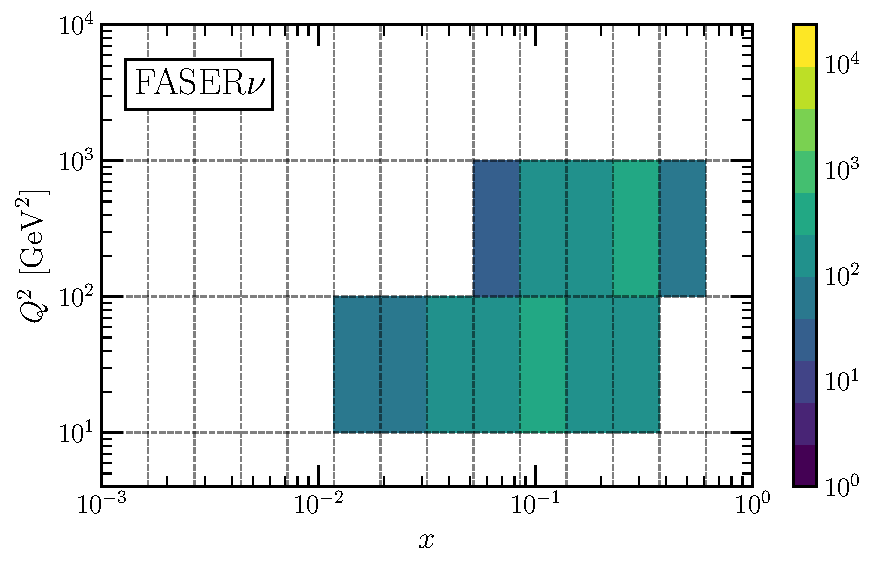
\includegraphics[width=0.495\textwidth]{plots/FPF-FASERv.pdf}
	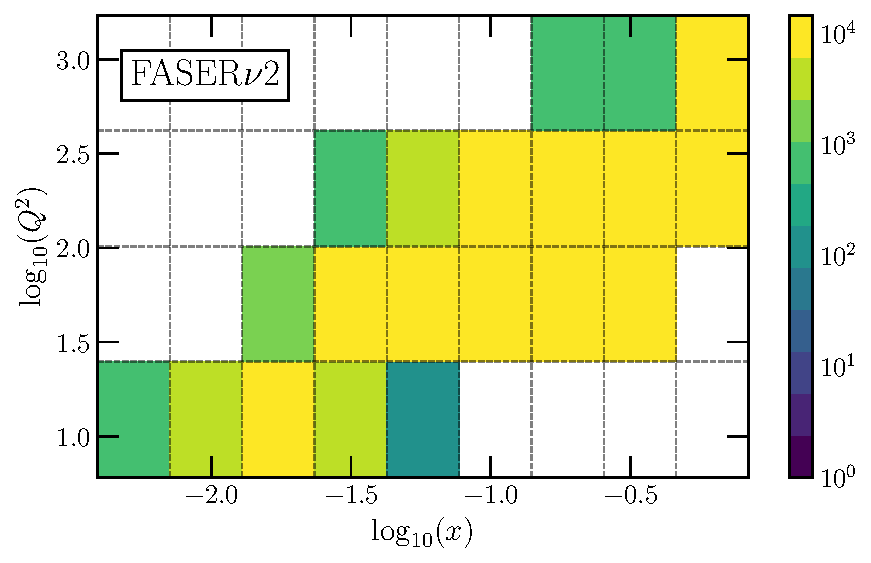
\includegraphics[width=0.495\textwidth]{plots/FPF-FASERv2.pdf}
	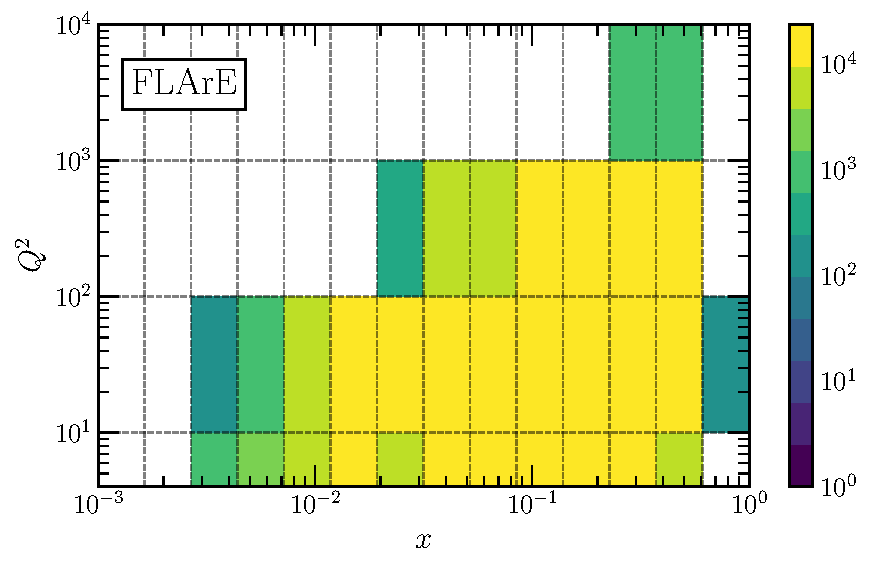
\includegraphics[width=0.495\textwidth]{plots/FPF-FLArE100.pdf}
	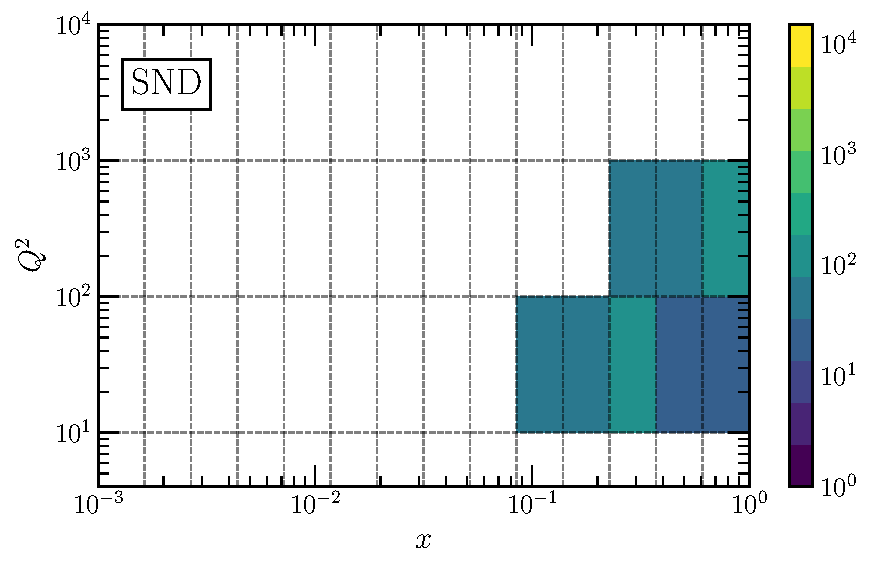
\includegraphics[width=0.495\textwidth]{plots/FPF-SND.pdf}
	\caption{\small The event yields per bin $N_{\rm ev}^{(i)}$, for muon neutrinos at the FASER$\nu$(2)
	and AdvSND detectors, and electron neutrinos the FLArE detector, restricted to the DIS region defined 
	by Eq.~(\ref{eq:DISconditions}).
	%
	Adding up all the bins in this plot results into the $N_{\nu_\mu}$ value listed in
	Table~\ref{tab:integrated_rates}.}
    \label{fig:fasernu2_muon}
\end{figure}
%-----------------------------------------------------------------------

Fig.~\ref{fig:fasernu2_muon} indicates
how the kinematic coverage of FASER$\nu$2 reaches
$x_{\rm min}\sim 3\times 10^{-3}$ at small-$x$ and $Q^2_{\rm max}\sim 2\times 10^3$
at large-$Q^2$, representing an extension
of around one order of magnitude in both directions as compared to available
DIS neutrino data on nuclear targets.
%
Fig.~\ref{fig:Kin_nNNPDF30_EIC_FPF} compares
the kinematic coverage of FASER$\nu$2 with that of electron-ion collisions
at the upcoming EIC~\cite{Khalek:2021ulf,AbdulKhalek:2021gbh}
and to other available hard-scattering datasets involving
nuclear targets or projectiles.
%
Specifically, we display the coverage of fixed-target neutral- and charged-current nuclear DIS,
fixed-target Drell-Yan production, and $W$, $Z$, $D$-meson, photon, and dijet
production in proton-lead collisions at the LHC entering the  nNNPDF3.0
determination~\cite{AbdulKhalek:2022fyi}.

%%%%%%%%%%%%%%%%%%%%%%%%%%%%%%%%%%%%%%%%%%%%%%%%%%%%%
\begin{figure}[t]
    \centering
    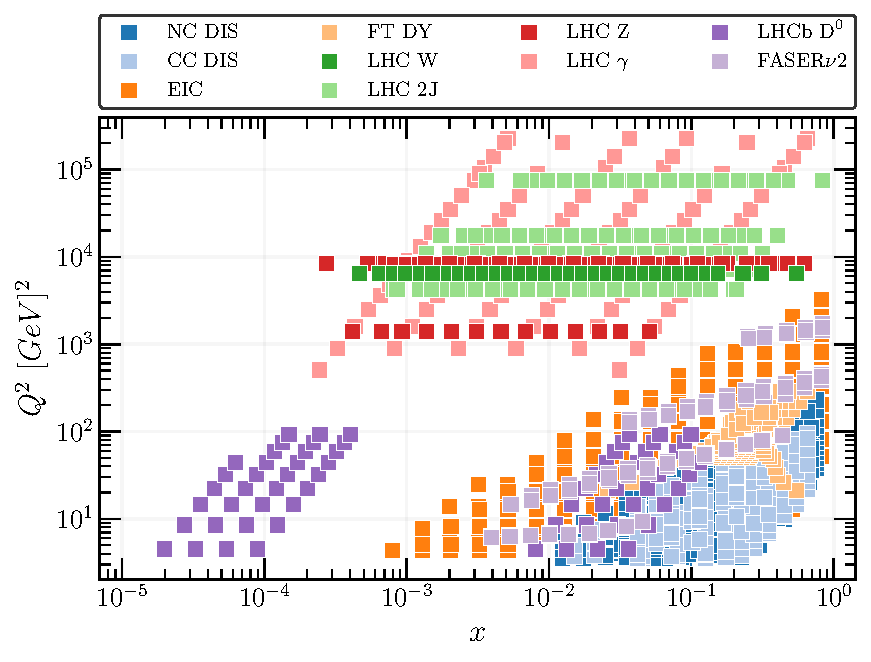
\includegraphics[width = 0.9\textwidth]{plots/Kin_nNNPDF30_EIC_FPF.pdf}
    \caption{The kinematic coverage of FASER$\nu$2 in the $(x,Q^2)$ plane,
      same as  Fig.~\ref{fig:fasernu2_muon},
      compared to that of electron-ion collisions
      at the EIC for the highest center-of-mass energies $\sqrt{s}$ planned,
      as well as to the coverage of other available hard-scattering datasets involving
      nuclear targets or projectiles.
      %
      Specifically, we display the coverage of fixed-target neutral- and charged-current nuclear DIS,
      fixed-target Drell-Yan production, and $W$, $Z$, $D$-meson, photon, and dijet
      production in proton-lead collisions at the LHC.
      }
    \label{fig:Kin_nNNPDF30_EIC_FPF}
\end{figure}
%%%%%%%%%%%%%%%%%%%%%%%%%%%%%%%%%%%%%%%%%%%%%%%%%%%%%%%%%%%%%

\subsection{Statistical and systematic uncertainties}
\label{subsec:uncertainties}

The event yields displayed in Fig.~\ref{fig:fasernu2_muon} for FASER$\nu$2, and the corresponding
calculations for the other experiments listed in Table~\ref{tab:FPF_experiments},
determine the associated statistical uncertainty in each bin
\be
\label{eq:statistical_uncertainties}
\delta^{\rm (stat)}  N_{\rm ev}^{(i)} = \sqrt{N_{\rm ev}^{(i)}} \, ,
\ee
such that the fractional statistical uncertainty per bin is $\delta^{\rm (stat)}_i=1/\sqrt{N_{\rm ev}^{(i)}}$.
%
Since we discard bins with less than 30 events, the fractional statistical uncertainty
ranges between $\lsim 1\%$ and $\sim 18\%$ for muon neutrinos in
the case of FASER$\nu$2 depending on the values of
$x$ and $Q^2$ associated to this bin.

%%%%%%%%%%%%%%%%%%%%%%%%%%%%%%%%%%%%%%%%%%%%%%%%%%%%%
\begin{figure}[h]
    \centering
    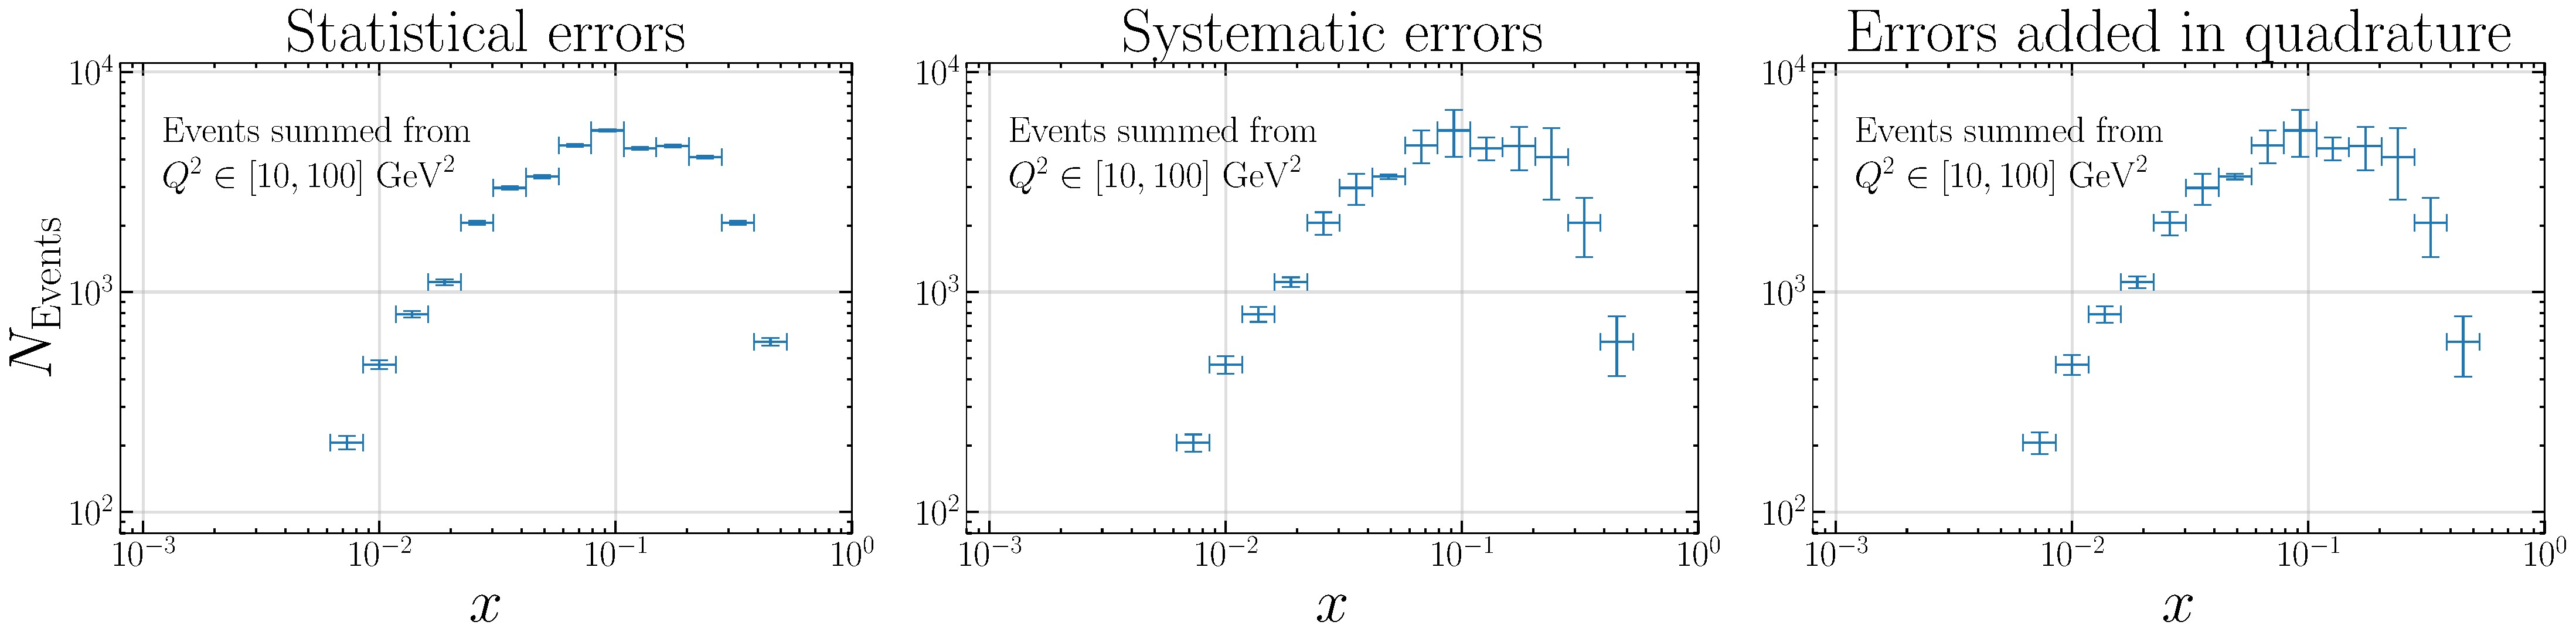
\includegraphics[width = 0.95\textwidth]{plots/error_plot_FASERv2_14.pdf}
    \caption{Same as Fig.~\ref{fig:fasernu2_muon} for FASER$\nu$2
      now as a function of $x$ after having integrated the event yields in the range $Q^2 \in [10,100]$ GeV$^2$.
      %
      In addition to the event yield values, we also show the error bars corresponding to
      statistical errors only (left), systematic errors only (middle), and the
      sum in quadrature of the two (right panel).
      %
      The error bars in the horizontal direction indicate the width of the adopted $x$-bins.
      }
    \label{fig:error_plot_FASERv2_14}
\end{figure}
%%%%%%%%%%%%%%%%%%%%%%%%%%%%%%%%%%%%%%%%%%%%%%%%%%%%%%%%%%%%%

These statistical uncertainties are displayed in the left panel
of Fig.~\ref{fig:error_plot_FASERv2_14}, which corresponds
to the same event yields as in
Fig.~\ref{fig:fasernu2_muon}
now as a function of $x$ after having integrated the event yields in the range $Q^2 \in [10,100]$ GeV$^2$.
%
The error bar in the vertical direction indicates the statistical uncertainties, while
that in the horizontal direction corresponds to the width of the $x$-bins.
%
Except for the bins with the smallest values of $x$, statistical uncertainties indeed
are at the percent level for FASER$\nu$2.

In addition to the statistical uncertainties given by Eq.~(\ref{eq:statistical_uncertainties}),
one needs to also estimate the systematic uncertainties associated to the
finite precision in the reconstruction
of the final state leptonic and hadronic variables listed in Table~\ref{tab:FPF_experiments}.
%
For instance, an event which would be classified into a given bin in $(x,Q^2,E_\nu)$ in the case
of a perfect detector may end up being
mis-classified into a different bin in the presence of systematic
shifts associated to the lepton energy $E_\ell$, lepton scattering angle $\theta_\ell$, and
hadronic energy $E_h$, as indicated by  Eq.~(\ref{eq:dis_kinematic_mapping}).

For each possible source of experimental systematic uncertainty, we therefore need to
quantify its impact at the event yield level.
%
In order to determine these bin-by-bin systematic uncertainties,
we extend the calculation delineated in Eq.~(\ref{sec:pseudo-data_generation}) as follows.
%
Let us consider for illustrative purposes the FASER${\nu}$2 case.
%
From Table~\ref{tab:FPF_experiments}, one reads that the detector
acceptance and reconstruction performance is specified by:
\bea
E_\ell \ge 100~{\rm GeV} \, , \quad \theta_\ell \le \tan^{-1}(0.5)\, , \qquad \nonumber\\
\delta E_\ell \sim 30\% \, 
 \quad \delta E_h \sim 30\% \, ,
 \ \, , \quad \delta\theta_\ell \sim 1~{\rm mrad} \, . 
\label{eq:fasernu2systematic_errors}
\eea
To translate the uncertainties in $\delta E_\ell$, $\delta E_h $,
and $\delta\theta_\ell$ into systematic errors associated to the event yields, 
\be
\label{eq:event_yields_systematic_error}
\delta_{\rm sys}^{(E_\ell)} N_{\rm ev}^{(i)} \, ,\quad
\delta_{\rm sys}^{(E_h)} N_{\rm ev}^{(i)}
\, ,\quad
\delta_{\rm sys}^{(\theta_\ell)} N_{\rm ev}^{(i)} \, ,\qquad i=1,\ldots,N_{\rm bin} \, ,
\ee
we generate first a Monte Carlo set of events, denoted by $\mathcal{D}_0$,
composed by $N_{\rm mc} = 10^7$ samples and determine the assignment of each event
to a point in the $\lp x,Q^2,E_{\nu}\rp$ space.
%
By integrating over this sample by means of Eq.~(\ref{MCintegration}) we determine
the binned event yields for this reference $\mathcal{D}_0$ sample.

We then produce a second Monte Carlo sample $\mathcal{D}_1$ starting from the events
of $\mathcal{D}_0$ which are then smeared with Gaussian distributions whose variances
are given by Eq.~(\ref{eq:fasernu2systematic_errors}).
%
The bin assignment of the events in the smeared sample $\mathcal{D}_1$ will
in general be different from those of the baseline sample.
%
The procedure is repeated $M$ times, leading to
$\mathcal{D}_k$ (with $k=1,\ldots,M$) smeared
samples each one leading to a different binned event yields
$ N_{\rm ev}^{(i)(k)}$.
%
Provided the number of samples $M$ is large enough,  {\color{red} the standard deviation over samples in this $ N_{\rm ev}^{(i)(k)}$
distribution}{\color{blue} $\rightarrow$ the average difference of events in the smeared datasets and the original dataset,$ N_{\rm ev}^{(i)(k>0)} -  N_{\rm ev}^{(i)(0)}$,} provides the sought-for estimate of the systematic uncertainties.
%
Furthermore, 
since the systematic errors are treated as uncorrelated among them,
by producing samples where only one source of error is varied at a time
we can determine the systematic errors Eq.~(\ref{eq:event_yields_systematic_error}) in each bin.

Fig.~\ref{fig:percentage_uncertainties_overview}
displays the systematic uncertainties associated
to $E_\ell$, $\theta_\ell$, and $E_h$.
in the  measurements
of the double-differential
neutrino scattering cross-section at FASER$\nu$2.
%
The magnitude of each systematic error is plotted as a function
of the average momentum fraction per bin $\la x\ra$
in three different bins of $Q^2$.
%
We indicate separately the results for neutrino and antineutrino projectiles as well as
those associated to inclusive and to charm production measurements.
%
Systematic uncertainties associated to the hadronic final state energy $E_h$ appear to be the largest.
%
The uncertainties associated to the charged lepton energy $E_\ell$ and scattering angle $\theta_\ell$ range
between a few percent up to 20\% in the nominal baseline scenario,
and in the case of the latter they are the smallest in the large-$x$ region.
%
The same procedure is adopted for all the experiments listed in Table~\ref{tab:FPF_experiments}.

%-----------------------------------------------------------------------
\begin{figure}[!ht]
  \centering
  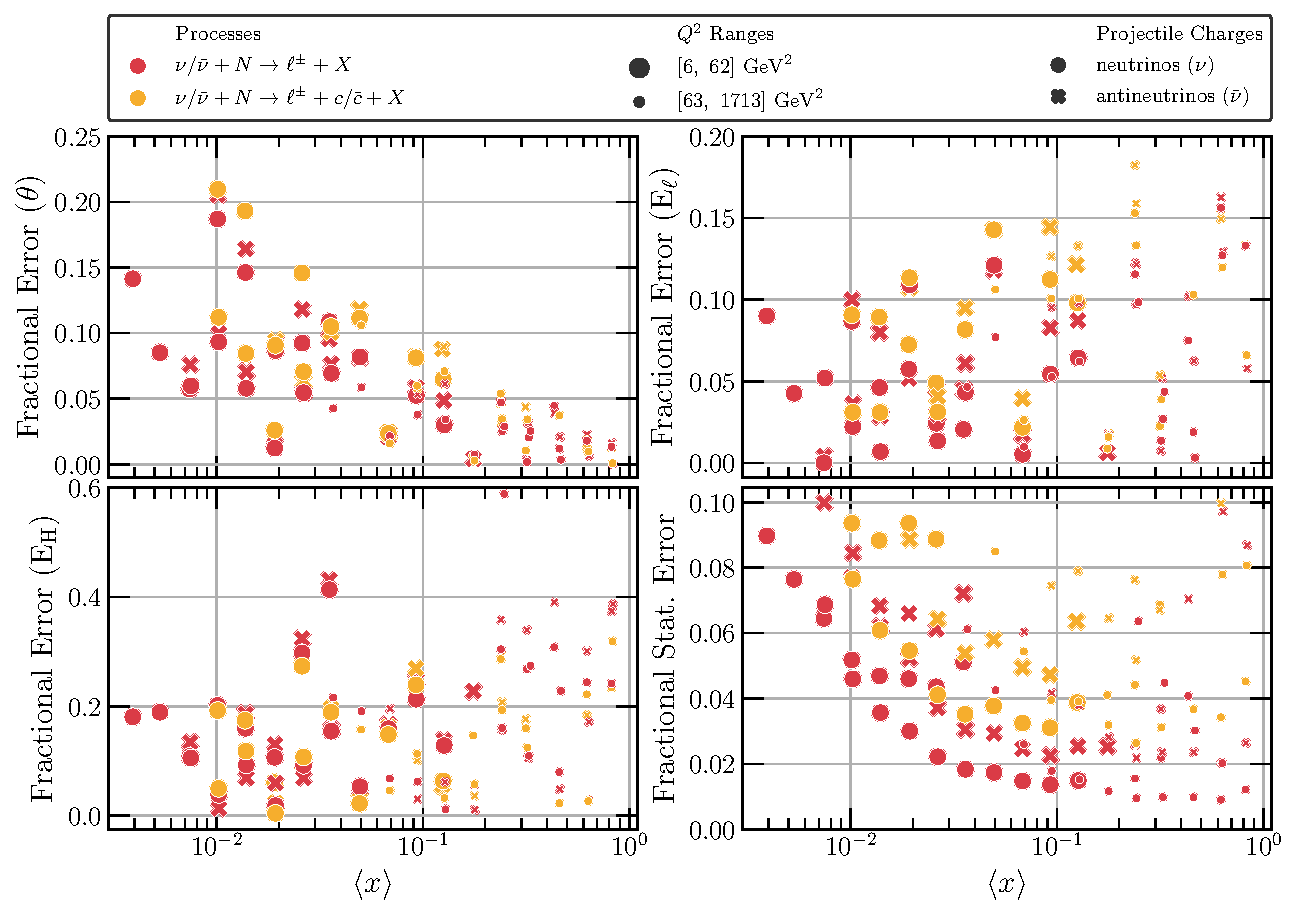
\includegraphics[width=\textwidth]{plots/percentage_errors.pdf}
  \caption{\small Estimated systematic uncertainties for the  measurements
    of the double-differential
    neutrino scattering cross-section at FASER$\nu$2.
    %
    We consider the systematic errors
    associated to the charged lepton energy $E_\ell$ and scattering angle $\theta_\ell$
    and to the hadronic energy $E_h$.
    %
    The size of each source of systematic error is plotted as a function
    of the average momentum fraction per bin $\la x\ra$
    in three different bins of $Q^2$.
    %
    We indicate separately the results for neutrino and antineutrino projectiles as well as
    those associated to inclusive and to charm production measurements.
  }
  \label{fig:percentage_uncertainties_overview}
\end{figure}
%-----------------------------------------------------------------------

The end result of the procedure is the estimate of statistical and systematic uncertainties
for each bin of the measurement, from which a experimental covariance matrix can be constructed as
\be
   {\rm cov}_{ij} = \delta_{ij} \lp \delta_{\rm stat}  N_{\rm ev}^{(i)}\rp^2
   + \lp \delta_{\rm sys}^{(E_\ell)} N_{\rm ev}^{(i)} \rp \lp \delta_{\rm sys}^{(E_\ell)} N_{\rm ev}^{(j)} \rp 
   + \lp \delta_{\rm sys}^{(E_h)} N_{\rm ev}^{(i)} \rp \lp\delta_{\rm sys}^{(E_h)} N_{\rm ev}^{(j)}\rp 
   + \lp \delta_{\rm sys}^{(\theta_\ell)} N_{\rm ev}^{(i)} \rp
   \lp \delta_{\rm sys}^{(\theta_\ell)} N_{\rm ev}^{(j)} \rp
   \, ,\qquad
 \nonumber
 \ee
 for $i,j=1,\ldots,N_{\rm bin}$, and the same for the associated correlation
 matrix of the measurement
 \be
 \rho_{ij} =  \frac{{\rm cov}_{ij}}{\sqrt{ {\rm cov}_{ii} }\sqrt{ {\rm cov}_{jj} } } \, . 
 \ee
 The relative covariance matrix, $ {\rm cov}_{ij}/( N_{\rm ev}^{(i)}N_{\rm ev}^{(j)})$, is
 independent of the considered observable and would also apply
 for the double-differential cross-sections Eqns.~(\ref{eq:neutrino_DIS_xsec_FL}) and~(\ref{eq:antineutrino_DIS_xsec_FL}) which are related to the event yields by a constant factor.
 
 One should emphasize that in a real experiment the actual covariance matrix will be
 composed by a much larger number of uncertainty sources, with typical
  HERA and LHC precision measurements characterised by up to hundreds
 of different sources of systematic error.
 %
 In particular, the assumption that a single source of systematic error, say $\delta E_\ell$,
 is fully correlated among all the bins in $(x,Q^2)$ is likely not to be realistic.
 %
 For this reason, here we present impact results both for the nominal correlation model,
 for the case where systematic and statistical uncertainties are added in quadrature,
 and intermediate scenarios.
  
 Fig.~\ref{fig:error_plot_FASERv2_14} (central and right panels) display
 the integrated event yields for FASER$\nu$2 as a function of $x$ for only
 systematic errors and for the sum in quadrature of statistical and systematic errors.
 %
 For most of the bins, for the baseline performance assumptions the total systematic
 uncertainty is at the $10\%$ and dominates over the statistical uncertainties.
 
 \subsection{Pseudo-data generation and impact on PDFs}

 In order to generate pseudo-data for double-differential
 neutrino scattering cross-sections at the LHC, we follow the procedure
 used for the HL-LHC PDF projections of~\cite{AbdulKhalek:2018rok} which was
 also adopted in~\cite{Ethier:2021ydt} and~\cite{Greljo:2021kvv} for SMEFT impact projections
 of vector-boson scattering and high-mass Drell-Yan data at the HL-LHC, respectively.
 %
 The starting point are the predictions for the differential neutrino scattering
 cross-section
 \be
 \label{eq:theory_dis_projections}
 \mathcal{O}_i^{{\rm (th)}} \equiv \frac{d^2\sigma^{\nu N}(x_i,Q^2_i,y_i)}{dxdy} \, ,\quad
 i=1,\ldots,N_{\rm bin} \, ,
 \ee
 with $(x_i,Q^2_i,y_i)$ being the corresponding bin centers.
 %
 The observables $\mathcal{O}_i $ are evaluated using {\sc\small YADISM} and {\sc\small PineAPPL}
 as described in Sect.~\ref{sec:settings}.
 %
 An important point here is the choice of PDF set entering the evaluation of
 the observable in Eq.~(\ref{eq:theory_dis_projections}): it should be consistent
 with that of the fitting framework used to assess their impact on the (n)PDFs.
 %
 For instance, when using the {\sc\small xFitter} profiling of PDF4LHC21, one needs
 to generate LHC neutrino pseudo-data also using PDF4LHC21 as input.
 %
 In order words, the generated pseudo-data should be fully consistent with the prior PDF
 set used as baseline, else one is introducing artificially inconsistencies which
 compromise the validity of the projection studies.
 
 The central values for the LHC neutrino scattering pseudo-data, denoted
 by $\mathcal{O}_i^{{\rm (exp)}} $, are obtained
 by fluctuating this reference theory prediction by the statistical and systematic
 uncertainties, that is
 \begin{equation}
  \label{eq:pseudo_data}
  \mathcal{O}_i^{{\rm (exp)}}
  =   \mathcal{O}_i^{{\rm (th)}}\left( 1+ r_{i} \delta_{i}^{\rm stat}
  + \sum_{k=E_\ell, E_h,\theta_\ell}
    r'_{k} \,\delta_{i,k}^{{\rm sys}}\right) \, , \qquad i=1,\ldots,N_{\rm bin} \, ,
 \end{equation}
 with $r_{i}$ and $r'_{k}$ being univariate Gaussian random numbers,
 and $\delta_i^{\rm stat}$ ($\delta_{i,k}^{\rm sys}$) indicate the relative statistical (systematic)
 uncertainties associated to the $i$-th bin (and $k$-th source of systematic uncertainty).
 %
 Note that a given systematic variation is assumed to be fully correlated among all the bins
 in the measurement.

 Alternatively, we can add all uncertainties in quadrature and account for a possible
 improvement in the systematic errors with respect to the current estimates,
 \be
 \delta_{i}^{\rm tot}
 = \left( \left( \delta_i^{\rm stat}\right)^2 + \sum_{k=1}^{n_{\rm sys}}
\left( \delta_{i,k}^{\rm sys} \right)^2\right)^{1/2} \, ,
 \ee
 and the pseudo-data is evaluated by means of
 \begin{equation}
  \label{eq:pseudo_data_v2}
  \mathcal{O}_i^{{\rm (exp)}}
  = \mathcal{O}_i^{{\rm (th)}}
    \left( 1+ r_i \delta_i^{\rm tot}
    \right) \,
    , \qquad i=1,\ldots,N_{\rm bin} \, .
 \end{equation}
 While the actual correlation model will lie somewhere between no correlation and full correlation,
 these two approaches to generate the pseudo-data bracket the projected impact
 on the PDFs and its dependence on the experimental correlation model.
 
In this section, we describe the analysis settings adopted to quantify
the impact of LHC neutrino measurements on the proton and nuclear PDFs.
%
First of all, we discuss the calculation of inclusive and charm structure functions
and their interpolation in terms of fast grids. 
%
Second, we review the Hessian profiling framework and how it is applied
in this work to proton and nuclear PDFs.
%
Third, we indicate the implementation of the LHC neutrino pseudo-data in the
NNPDF framework and the settings of the subsequent global PDF analysis.

The procedure described in Sect.~\ref{sec:dis_pseudodata} returns
$N_{\rm bin}$ bins of LHC neutrino pseudo-data $\mathcal{O}_i^{{\rm (exp)}}$, Eq.~(\ref{eq:pseudo_data}), covering the $(x,Q^2,E_\nu)$ kinematic region accessible by the experiment,
together with the associated statistical and systematic uncertainties.
%
The calculation of this pseudo-data relies on the corresponding set of
theoretical predictions for the same observables $\mathcal{O}_i^{{\rm (th)}}$,
Eq.~(\ref{eq:theory_dis_projections}).
%
Here we evaluate inclusive and charm DIS structure functions with the
{\sc\small YADISM}~\cite{yadism,Candido:2023utz} program
interfaced to {\sc\small PineAPPL}~\cite{Carrazza:2020gss, christopher_schwan_2023_7995675}
to return a fast interpolation grid admitting a generic PDF input.
%
DGLAP evolution effects between the scale $Q_0$ at which PDFs are evaluated
and the data scale $Q$ are provided by {\sc\small EKO}~\cite{Candido:2022tld}.

The resulting {\sc\small PineAPPL} grids provide a fast evaluation
of Eq.~(\ref{eq:theory_dis_projections}) for an arbitrary choice of the
input PDFs at the initial scale $Q_0$, with the latter accessed via their
{\sc\small LHAPDF} interface~\cite{Buckley:2014ana}.
%
Whenever pseudo-data is generated, it is crucial to adopt common inputs with
the subsequent PDF analysis.
%
For instance, if one aims to include the LHC neutrino data into the NNPDF4.0
NNLO determination, $\mathcal{O}_i^{{\rm (th)}}$ must be evaluated also at NNLO
and also using
NNPDF4.0 as input for consistency, else artificial tensions between theory
and data would be introduced during the fit biasing the results.

By means of this theoretical pipeline, predictions for
DIS inclusive structure functions on an isoscalar target $N$ are computed
using
\be
\label{eq:neutrino_DIS_xsec}
\frac{d^2\sigma^{\nu N}(x,Q^2,y)}{dxdy} =  \frac{G_F^2s/4\pi}{\lp 1+Q^2/m_W^2\rp^2}\lc Y_+F^{\nu N}_2(x,Q^2) - y^2F^{\nu N}_L(x,Q^2) +Y_- xF^{\nu N}_3(x,Q^2)\rc  \, ,
\ee
with an analogous formula for antineutrino scattering with the sign of $xF_3$ flipped.
%
A {\sc\small PineAPPL} interpolation grid for
Eq.~(\ref{eq:neutrino_DIS_xsec}) is evaluated at the $(x,Q^2,E_\nu)$ bins
for which pseudo-data is generated using DGLAP evolution and coefficient
functions at $\mathcal{O}\lp \alpha_s^2\rp$ and accounting for target mass effects.
%
No higher-twists corrections to the structure functions are included, since we cut
data with $W^2 \ge 12.5$ GeV in order to suppress them.
%
Deviations from isoscalarity and nuclear modifications with respect
to a free isoscalar target are accounted for at the input PDF level,
leaving the grid entering the evaluation of Eq.~(\ref{eq:neutrino_DIS_xsec}) unchanged.
%
No heavy quark mass effects are considered for at the level of these inclusive structure functions.

Concerning charm structure functions, for experiments with charm tagging
capabilities theoretical predictions are evaluated for
\be
\label{eq:neutrino_DIS_xsec}
\frac{d^2\sigma^{\nu N}_c(x,Q^2,y)}{dxdy} =  \frac{G_F^2s/4\pi}{\lp 1+Q^2/m_W^2\rp^2}\lc Y_+F_{2,c}^{\nu N}(x,Q^2) - y^2F^{\nu N}_{L,c}(x,Q^2) +Y_- xF^{\nu N}_{3,c}(x,Q^2)\rc  \, ,
\ee
with the DIS charm structure functions evaluated in the FONLL general-mass variable-flavour-number
scheme~\cite{Forte:2010ta,Ball:2011mu,Faura:2020oom} in order to account for charm mass effects.
%
Eq.~(\ref{eq:neutrino_DIS_xsec}) is computed with $\mathcal{O}\lp \alpha_s^2\rp$ massless
coefficient functions and $\mathcal{O}\lp \alpha_s\rp$ massive ones, given
that the $\mathcal{O}\lp \alpha_s^2\rp$ massive calculation~\cite{Gao:2017kkx} is not publicly available.
%
Nevertheless, the $\mathcal{O}\lp \alpha_s\rp$ massive coefficient functions
encapsulate the dominant charm mass dependence of the double differential
cross-section.
%
We assume 100\% efficiency in charm tagging and do not impose acceptance cuts on the charm
quark or $D$-meson kinematics (the only acceptance requirements are applied to the final-state
charged lepton, as indicated in  Table~\ref{tab:FPF_experiments}).

We note that experiments without charm-tagging capabilities can still identify charm production
events by means of the dimuon final state,
\be
\nu + N \to \mu^+ + c~(\to D) + X \to \mu^+ + \mu^- +X \, ,
\ee
by profiting from the semileptonic decays of the $D$-meson leading
to the characteristic signature of two opposite-sign muons.
%
In this case, the  differential charm production cross-section Eq.~(\ref{eq:neutrino_DIS_xsec})
must be accompanied by the corresponding branching ratio
\be
\frac{d^2\sigma^{\nu N}_c(x,Q^2,y)}{dxdy}\mathcal{B}\lp c \to D \to \mu + X\rp \, ,
\ee
which given that $\mathcal{B}\sim 10\%$ suppresses the reconstructed charm
production event yields by around an order of magnitude.
%
For experiments reconstructing the dimuon final state,
we also apply the muon acceptance criteria to both muons.


In this work we consider two complementary approaches in order to assess the
impact of LHC neutrino data on the proton and nuclear PDFs.
%
On the one hand, the Hessian profiling of a prior proton or
nuclear PDF set, which here are taken to be PDF4LHC21~\cite{PDF4LHCWorkingGroup:2022cjn} and
EPPS21~\cite{Eskola:2021nhw} respectively.
%
On the other hand, the inclusion of the LHC neutrino structure functions
on the NNPDF global analysis framework~\cite{NNPDF:2021uiq,NNPDF:2021njg}.
%
Here we summarise the details of the Hessian profiling procedure and
outline how it is applied in our work.

The profiling method applied to Hessian PDF fits is described in~\cite{Paukkunen:2014zia, Schmidt:2018hvu, AbdulKhalek:2018rok, HERAFitterdevelopersTeam:2015cre} and is based
on minimizing a goodness-of-fit error function defined as
\begin{equation}
\chi^2 = 
\sum_{i=1}^{N_{\textrm{bin}}} 
\frac{\left(  \mathcal{O}_i^{\rm (exp)}
            + \Gamma_i^{\alpha,\textrm{pd}}
              b_\alpha^{\textrm{(pd)}}
            - \mathcal{O}_i^{\rm (th)}
            - \Gamma_i^{\beta,\textrm{th}}
              b_\beta^{(\textrm{th})}
     \right)^2
     }{ \left(\delta_i^{\rm stat}\right)^2 }
+ \sum_\alpha \lp b_\alpha^{(\textrm{pd})}\rp^2
+ \sum_\beta  \lp b_\beta^{\textrm{(th)}}\rp ^2 \, .
\label{eq:profilingchi2}
\end{equation}
The pseudodata 
$\mathcal{O}_i^{\rm (exp)}$ 
is obtained from the central theoretical prediction 
$\mathcal{O}_i^{(\textrm{th})}$
for each bin $i$ out of $N_{\textrm{bin}}$ by fluctuating
it within its uncertainties, following either
Eq.~(\ref{eq:pseudo_data}), when accounting for the correlations
between systematic uncertainties, or Eq.~(\ref{eq:pseudo_data_v2}),
in the case in which errors are added in quadrature.

The correlated uncertainties for the pseudodata and for the theoretical prediction 
are contained in the nuisance parameter vectors $b^{(\textrm{pd})}$ and $b^{(\textrm{th})}$, respectively, and the total uncorrelated uncertainties are denoted by $\delta_{{\rm stat},i}$.
%
The effect of the nuisance parameters
on the observables $\mathcal{O}_i^{\rm (exp)}$ and $\mathcal{O}_i^{\rm (th)}$
is described by the matrices $\Gamma_i^{\textrm{pd}}$ and $\Gamma_i^{\textrm{th}}$.
%
The indices $\alpha$ and $\beta$ then run over the uncertainty nuisance parameters for the pseudodata and the theoretical prediction, respectively.
%
The nuisance parameter values $b_\beta^{\textrm{(th,min)}}$ that minimize Eq.~\eqref{eq:profilingchi2} give the central PDFs $f'_0$ optimized to the profiled dataset in the form
\begin{equation}
f_0' = f_0
      + \sum_\beta b_\beta^{\textrm{(th,min)}} 
        \left(  \frac{f_\beta^+   -  f_\beta^- }{2}
              -    b_\beta^{\textrm{(th,min)}}
                \frac{f_\beta^+ + f_\beta^- - 2f_0}{2}
        \right),
\end{equation}
where $f_0$ is the original central PDF and the up and down variation eigenvectors are given by $f^+, f^-$.
%
The reduction in the uncertainties of the profiled PDFs indicate the impact
of the projected data with respect to the assumed prior PDF set.


The profiling studies carried out in this work are performed using v2.2.1 of the \textsc{xFitter} open-source QCD analysis framework~\cite{Alekhin:2014irh, Bertone:2017tig, xFitter:2022zjb, xFitter:web}.
%
To this end, a new interface between  {\sc\small PineAPPL} and {\sc\small xFitter} has been developed and is available in {\sc\small xFitter}.
%
All the experimental and theoretical data files used in the analysis, including
the  {\sc\small PineAPPL}  grids, are available
from the {\sc\small xFitter} repository.




